\chapter{File System Implementation}

\section{Introduction}

A file system is responsible for organizing, storing, retrieving, protecting, and managing data on storage devices. File system implementation determines how files are represented on disk, how free space is tracked, and how reliability is maintained.

Modern file systems must provide:

\begin{itemize}
\item Efficient storage utilization
\item Fast file access
\item Reliability and recovery
\item Scalability
\item Security and permissions
\end{itemize}

\section{File System Architecture}

A typical file system consists of several layers.

\begin{figure}[H]
\centering
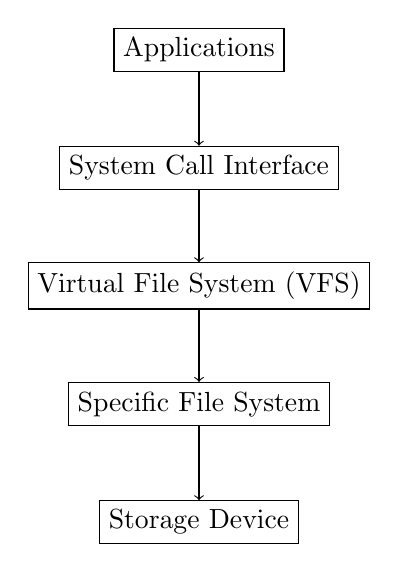
\begin{tikzpicture}
\node[draw] (app) at (0,6) {Applications};
\node[draw] (api) at (0,4.5) {System Call Interface};
\node[draw] (vfs) at (0,3) {Virtual File System (VFS)};
\node[draw] (fs) at (0,1.5) {Specific File System};
\node[draw] (disk) at (0,0) {Storage Device};

\draw[->] (app)--(api);
\draw[->] (api)--(vfs);
\draw[->] (vfs)--(fs);
\draw[->] (fs)--(disk);
\end{tikzpicture}
\caption{Layered File System Architecture}
\end{figure}

Responsibilities include:

\begin{itemize}
\item Namespace management
\item Metadata management
\item Data allocation
\item Caching
\item Recovery
\end{itemize}

\section{On-Disk Structures}

On-disk structures persist across system reboots.

Common structures include:

\begin{itemize}
\item Boot Block
\item Superblock
\item Inode Table
\item Data Blocks
\item Journals
\item Free Space Information
\end{itemize}

\begin{figure}[H]
\centering
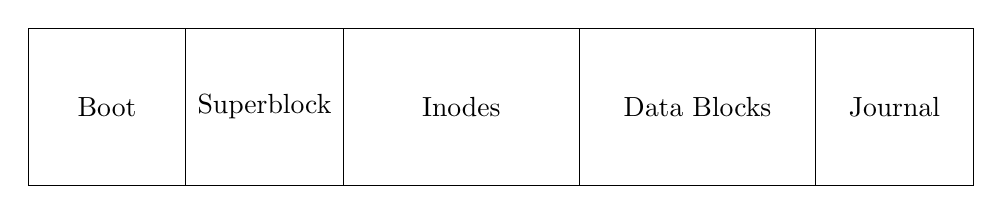
\begin{tikzpicture}
\draw (0,0) rectangle (12,2);

\draw (2,0)--(2,2);
\draw (4,0)--(4,2);
\draw (7,0)--(7,2);
\draw (10,0)--(10,2);

\node at (1,1) {Boot};
\node at (3,1) {Superblock};
\node at (5.5,1) {Inodes};
\node at (8.5,1) {Data Blocks};
\node at (11,1) {Journal};
\end{tikzpicture}
\caption{Typical On-Disk Layout}
\end{figure}

\section{In-Memory Structures}

To improve performance, operating systems maintain memory-resident structures.

Examples:

\begin{itemize}
\item Mount table
\item Buffer cache
\item Open file table
\item Directory cache
\item Inode cache
\end{itemize}

\section{Boot Block}

The boot block resides at the beginning of the storage device.

Purpose:

\begin{itemize}
\item Contains bootstrap code
\item Used during system startup
\item Loads operating system kernel
\end{itemize}

\section{Superblock}

The superblock stores global file system metadata.

Typical contents:

\begin{itemize}
\item File system size
\item Block size
\item Free block count
\item Free inode count
\item Mount information
\item File system state
\end{itemize}

\begin{table}[H]
\centering
\begin{tabular}{ll}
\toprule
Field & Description \\
\midrule
Block Size & Size of disk block \\
Total Blocks & Total blocks in file system \\
Free Blocks & Available blocks \\
Inode Count & Number of inodes \\
State & Clean/Dirty state \\
\bottomrule
\end{tabular}
\caption{Typical Superblock Fields}
\end{table}

\section{Inodes}

An inode is a data structure describing a file.

An inode stores:

\begin{itemize}
\item Ownership
\item Permissions
\item File size
\item Timestamps
\item Block pointers
\end{itemize}

An inode does not store the filename.

\begin{figure}[H]
\centering
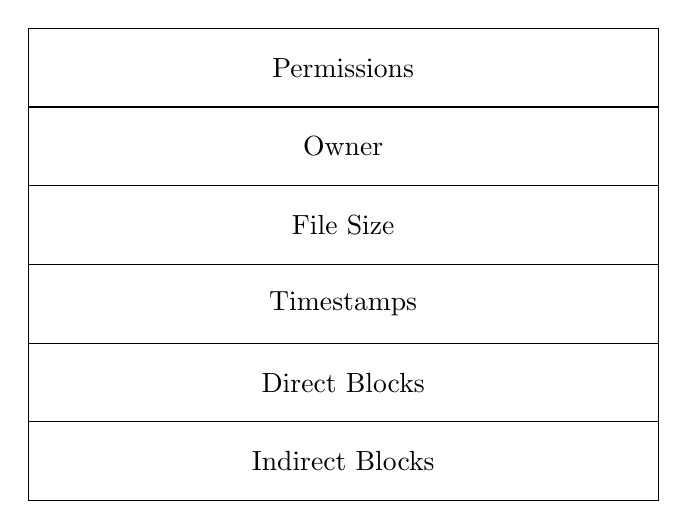
\begin{tikzpicture}
\draw (0,0) rectangle (8,6);

\draw (0,5)--(8,5);
\draw (0,4)--(8,4);
\draw (0,3)--(8,3);
\draw (0,2)--(8,2);
\draw (0,1)--(8,1);

\node at (4,5.5) {Permissions};
\node at (4,4.5) {Owner};
\node at (4,3.5) {File Size};
\node at (4,2.5) {Timestamps};
\node at (4,1.5) {Direct Blocks};
\node at (4,0.5) {Indirect Blocks};
\end{tikzpicture}
\caption{Simplified Inode Structure}
\end{figure}

\section{File Control Blocks}

A File Control Block (FCB) stores file metadata.

Information includes:

\begin{itemize}
\item File attributes
\item Location
\item Ownership
\item Access rights
\end{itemize}

Unix systems typically use inodes instead of traditional FCBs.

\section{Allocation Methods}

Allocation methods determine how file data is placed on disk.

Three classic methods:

\begin{itemize}
\item Contiguous Allocation
\item Linked Allocation
\item Indexed Allocation
\end{itemize}

\section{Contiguous Allocation}

File occupies consecutive disk blocks.

Example:

\[
File\ A \rightarrow Blocks\ 20-29
\]

\begin{figure}[H]
\centering
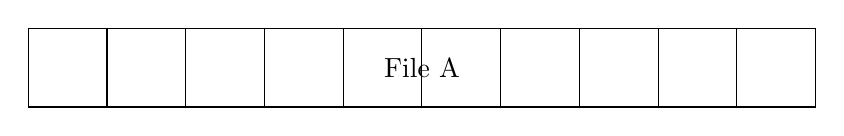
\begin{tikzpicture}
\draw (0,0) rectangle (10,1);

\foreach \x in {1,2,3,4,5,6,7,8,9}
{
\draw (\x,0)--(\x,1);
}

\node at (5,0.5) {File A};
\end{tikzpicture}
\caption{Contiguous Allocation}
\end{figure}

Advantages:

\begin{itemize}
\item Fast sequential access
\item Fast random access
\end{itemize}

Disadvantages:

\begin{itemize}
\item External fragmentation
\item Difficult file growth
\end{itemize}

\section{Linked Allocation}

Each block contains pointer to next block.

\begin{figure}[H]
\centering
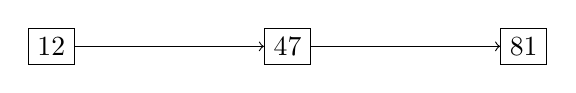
\begin{tikzpicture}
\node[draw] (a) at (0,0) {12};
\node[draw] (b) at (3,0) {47};
\node[draw] (c) at (6,0) {81};

\draw[->] (a)--(b);
\draw[->] (b)--(c);
\end{tikzpicture}
\caption{Linked Allocation}
\end{figure}

Advantages:

\begin{itemize}
\item No external fragmentation
\item Easy growth
\end{itemize}

Disadvantages:

\begin{itemize}
\item Poor random access
\item Pointer overhead
\end{itemize}

\section{Indexed Allocation}

A special index block contains addresses of all file blocks.

\begin{figure}[H]
\centering
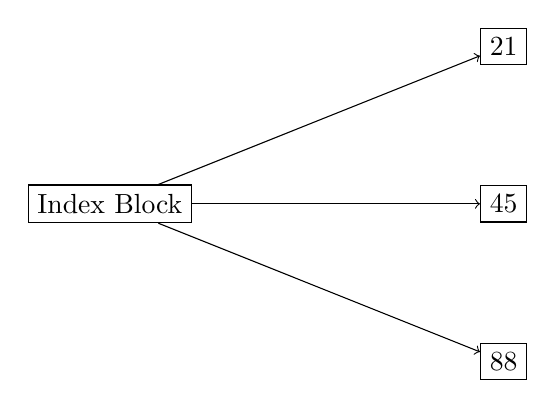
\begin{tikzpicture}
\node[draw] (index) at (0,0) {Index Block};

\node[draw] (b1) at (5,2) {21};
\node[draw] (b2) at (5,0) {45};
\node[draw] (b3) at (5,-2) {88};

\draw[->] (index)--(b1);
\draw[->] (index)--(b2);
\draw[->] (index)--(b3);
\end{tikzpicture}
\caption{Indexed Allocation}
\end{figure}

Advantages:

\begin{itemize}
\item Efficient random access
\item No external fragmentation
\end{itemize}

Disadvantages:

\begin{itemize}
\item Index overhead
\item Additional block accesses
\end{itemize}

\section{Free Space Management}

The operating system tracks unused disk blocks.

Requirements:

\begin{itemize}
\item Fast allocation
\item Fast deallocation
\item Low overhead
\end{itemize}

Common techniques:

\begin{itemize}
\item Bitmaps
\item Free Lists
\end{itemize}

\section{Bitmaps}

Each block is represented by one bit.

\[
0 = Free
\]

\[
1 = Allocated
\]

Example:

\[
111001010000111
\]

Advantages:

\begin{itemize}
\item Compact
\item Efficient searching
\end{itemize}

\begin{figure}[H]
\centering
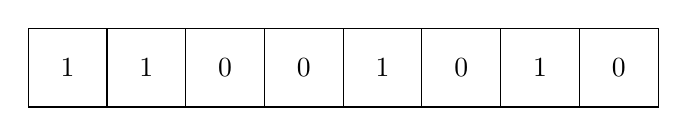
\begin{tikzpicture}
\draw (0,0) rectangle (8,1);

\foreach \x in {1,2,3,4,5,6,7}
{
\draw (\x,0)--(\x,1);
}

\node at (0.5,0.5) {1};
\node at (1.5,0.5) {1};
\node at (2.5,0.5) {0};
\node at (3.5,0.5) {0};
\node at (4.5,0.5) {1};
\node at (5.5,0.5) {0};
\node at (6.5,0.5) {1};
\node at (7.5,0.5) {0};
\end{tikzpicture}
\caption{Bitmap Free Space Tracking}
\end{figure}

\section{Free Lists}

Free blocks are linked together.

Example:

\[
14 \rightarrow 27 \rightarrow 65 \rightarrow 102
\]

Advantages:

\begin{itemize}
\item Simple implementation
\end{itemize}

Disadvantages:

\begin{itemize}
\item Slower search
\item Poor locality
\end{itemize}

\section{Journaling}

Journaling improves reliability.

Before modifying metadata:

\begin{enumerate}
\item Write operation to journal
\item Commit journal entry
\item Apply actual changes
\end{enumerate}

Advantages:

\begin{itemize}
\item Faster recovery
\item Reduced corruption
\end{itemize}

\begin{figure}[H]
\centering
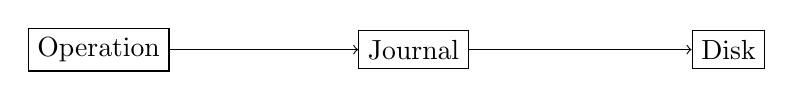
\begin{tikzpicture}
\node[draw] (op) at (0,0) {Operation};
\node[draw] (journal) at (4,0) {Journal};
\node[draw] (disk) at (8,0) {Disk};

\draw[->] (op)--(journal);
\draw[->] (journal)--(disk);
\end{tikzpicture}
\caption{Journaling Workflow}
\end{figure}

\section{Log Structured File Systems}

Log Structured File Systems (LFS) treat storage as an append-only log.

Characteristics:

\begin{itemize}
\item Sequential writes
\item Better write performance
\item Crash recovery support
\end{itemize}

Challenges:

\begin{itemize}
\item Cleaning old segments
\item Space reclamation
\end{itemize}

\section{ext4 Overview}

ext4 is one of the most widely used Linux file systems.

Features:

\begin{itemize}
\item Journaling
\item Extents
\item Delayed allocation
\item Large file support
\item Fast fsck
\end{itemize}

Advantages:

\begin{itemize}
\item Mature
\item Reliable
\item High performance
\end{itemize}

\section{NTFS Overview}

NTFS is the default Windows file system.

Features:

\begin{itemize}
\item Journaling
\item Access Control Lists
\item Compression
\item Encryption
\item Large volume support
\end{itemize}

Central structure:

\begin{itemize}
\item Master File Table (MFT)
\end{itemize}

\section{File System Consistency}

Consistency means metadata correctly reflects file system state.

Potential issues:

\begin{itemize}
\item Power failure
\item Kernel crash
\item Incomplete writes
\end{itemize}

Consistency mechanisms:

\begin{itemize}
\item Journaling
\item Checksums
\item Recovery tools
\end{itemize}

\section{fsck Overview}

fsck (File System Check) repairs inconsistent file systems.

Responsibilities:

\begin{itemize}
\item Verify metadata
\item Repair inode errors
\item Recover orphaned files
\item Correct allocation maps
\end{itemize}

Typical checks:

\begin{enumerate}
\item Superblock validation
\item Inode validation
\item Block consistency
\item Directory consistency
\item Reference count verification
\end{enumerate}

\section{Dedicated Interview Section: How Linux Stores Files Internally}

Linux stores files using inodes.

When a file is created:

\begin{enumerate}
\item Allocate inode
\item Allocate data blocks
\item Create directory entry
\item Associate filename with inode number
\end{enumerate}

Example:

\begin{figure}[H]
\centering
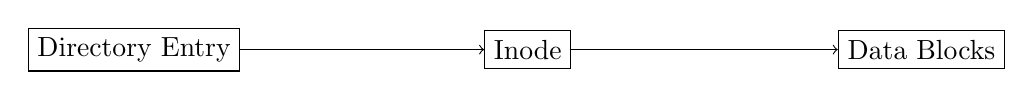
\begin{tikzpicture}
\node[draw] (dir) at (0,0) {Directory Entry};

\node[draw] (inode) at (5,0) {Inode};

\node[draw] (data) at (10,0) {Data Blocks};

\draw[->] (dir)--(inode);
\draw[->] (inode)--(data);
\end{tikzpicture}
\caption{Linux File Storage Path}
\end{figure}

Important interview fact:

\begin{itemize}
\item Filename is stored in directory entries.
\item Metadata is stored in inode.
\item Actual contents are stored in data blocks.
\end{itemize}

\section{Allocation Method Comparison}

\begin{table}[H]
\centering
\begin{tabular}{llll}
\toprule
Method & Random Access & Growth & Fragmentation \\
\midrule
Contiguous & Excellent & Poor & External \\
Linked & Poor & Excellent & None \\
Indexed & Good & Good & None \\
\bottomrule
\end{tabular}
\caption{Allocation Method Comparison}
\end{table}

\section{Key Takeaways}

\begin{keytakeaways}
File systems organize data using on-disk and in-memory structures. Important on-disk structures include the boot block, superblock, inode table, data blocks, and journals. Files may be allocated using contiguous, linked, or indexed allocation. Linux stores metadata in inodes and filenames in directory entries. Journaling improves reliability and enables rapid crash recovery. ext4 and NTFS are modern journaling file systems with advanced allocation and consistency mechanisms.
\end{keytakeaways}

\section{Interview Questions with Answers}

\begin{enumerate}
\item What is a file system?\\
A mechanism for organizing and managing files on storage devices.

\item What is a superblock?\\
A structure containing global file system metadata.

\item What is an inode?\\
A structure describing a file's metadata.

\item Does an inode store filenames?\\
No.

\item Where are filenames stored?\\
Directory entries.

\item What is a boot block?\\
Storage area containing bootstrap code.

\item What are on-disk structures?\\
Persistent file system structures stored on storage devices.

\item What are in-memory structures?\\
Runtime file system data structures.

\item What is contiguous allocation?\\
Allocating consecutive disk blocks.

\item Advantage of contiguous allocation?\\
Fast access.

\item Disadvantage of contiguous allocation?\\
External fragmentation.

\item What is linked allocation?\\
Blocks linked through pointers.

\item Advantage of linked allocation?\\
Easy file growth.

\item Disadvantage of linked allocation?\\
Poor random access.

\item What is indexed allocation?\\
Using an index block to locate data blocks.

\item What is a bitmap?\\
Bit-based free space tracking mechanism.

\item What is journaling?\\
Logging updates before applying them.

\item Why is journaling useful?\\
Crash recovery.

\item What is a log-structured file system?\\
A file system that writes data sequentially as a log.

\item What is ext4?\\
A widely used Linux journaling file system.

\item What is NTFS?\\
Windows' default file system.

\item What is the MFT?\\
Master File Table in NTFS.

\item What is file system consistency?\\
Correct metadata and storage state.

\item What is fsck?\\
A file system repair utility.

\item How does Linux store files internally?\\
Directory entry $\rightarrow$ inode $\rightarrow$ data blocks.
\end{enumerate}

\section{MCQs with Answers}

\begin{enumerate}
\item Which structure stores global file system metadata?
\begin{enumerate}[label=(\alph*)]
\item Inode
\item Superblock
\item Bitmap
\item Journal
\end{enumerate}
Answer: (b)

\item Linux file metadata is stored in:
\begin{enumerate}[label=(\alph*)]
\item Directories
\item Inodes
\item Bitmaps
\item Journals
\end{enumerate}
Answer: (b)

\item File names are stored in:
\begin{enumerate}[label=(\alph*)]
\item Inodes
\item Data Blocks
\item Directory Entries
\item Journals
\end{enumerate}
Answer: (c)

\item Which allocation method provides best random access?
\begin{enumerate}[label=(\alph*)]
\item Linked
\item Contiguous
\item Chained
\item Free List
\end{enumerate}
Answer: (b)

\item Linked allocation stores:
\begin{enumerate}[label=(\alph*)]
\item Pointers
\item Inodes
\item Journals
\item Bitmaps
\end{enumerate}
Answer: (a)

\item Indexed allocation uses:
\begin{enumerate}[label=(\alph*)]
\item FAT
\item Bitmap
\item Index Block
\item Cache
\end{enumerate}
Answer: (c)

\item A bitmap tracks:
\begin{enumerate}[label=(\alph*)]
\item Directories
\item Inodes
\item Free Space
\item Permissions
\end{enumerate}
Answer: (c)

\item Journaling improves:
\begin{enumerate}[label=(\alph*)]
\item Recovery
\item CPU Speed
\item Network Performance
\item Scheduling
\end{enumerate}
Answer: (a)

\item ext4 supports:
\begin{enumerate}[label=(\alph*)]
\item Journaling
\item Extents
\item Delayed Allocation
\item All of the Above
\end{enumerate}
Answer: (d)

\item NTFS uses:
\begin{enumerate}[label=(\alph*)]
\item MFT
\item FAT
\item inode2
\item extents only
\end{enumerate}
Answer: (a)

\item fsck is used for:
\begin{enumerate}[label=(\alph*)]
\item Scheduling
\item Memory Management
\item File System Repair
\item Paging
\end{enumerate}
Answer: (c)

\item Which allocation method suffers external fragmentation?
\begin{enumerate}[label=(\alph*)]
\item Contiguous
\item Linked
\item Indexed
\item Bitmap
\end{enumerate}
Answer: (a)

\item A boot block contains:
\begin{enumerate}[label=(\alph*)]
\item Bootstrap Code
\item Data Blocks
\item Directories
\item MFT
\end{enumerate}
Answer: (a)

\item Linked allocation offers:
\begin{enumerate}[label=(\alph*)]
\item Excellent Random Access
\item Easy Growth
\item No Metadata
\item No Pointers
\end{enumerate}
Answer: (b)

\item Which structure stores block pointers?
\begin{enumerate}[label=(\alph*)]
\item Journal
\item Inode
\item Bitmap
\item Boot Block
\end{enumerate}
Answer: (b)

\item ext4 is primarily associated with:
\begin{enumerate}[label=(\alph*)]
\item Linux
\item Windows
\item macOS
\item BIOS
\end{enumerate}
Answer: (a)

\item NTFS is primarily associated with:
\begin{enumerate}[label=(\alph*)]
\item Linux
\item Android
\item Windows
\item BSD
\end{enumerate}
Answer: (c)

\item Which method uses one bit per block?
\begin{enumerate}[label=(\alph*)]
\item Linked List
\item Bitmap
\item Journal
\item MFT
\end{enumerate}
Answer: (b)

\item Journaling writes updates first to:
\begin{enumerate}[label=(\alph*)]
\item RAM
\item Journal
\item CPU Cache
\item Boot Block
\end{enumerate}
Answer: (b)

\item Which utility repairs corrupted file systems?
\begin{enumerate}[label=(\alph*)]
\item ls
\item grep
\item fsck
\item chmod
\end{enumerate}
Answer: (c)

\item File data is stored in:
\begin{enumerate}[label=(\alph*)]
\item Data Blocks
\item Inodes
\item Directories
\item Journals
\end{enumerate}
Answer: (a)

\item In-memory structures improve:
\begin{enumerate}[label=(\alph*)]
\item Performance
\item Power Usage
\item BIOS Speed
\item Interrupt Rate
\end{enumerate}
Answer: (a)

\item Log-structured file systems emphasize:
\begin{enumerate}[label=(\alph*)]
\item Sequential Writes
\item Random Writes Only
\item No Logging
\item FAT Tables
\end{enumerate}
Answer: (a)

\item Metadata includes:
\begin{enumerate}[label=(\alph*)]
\item Ownership
\item Permissions
\item Timestamps
\item All of the Above
\end{enumerate}
Answer: (d)

\item Linux file lookup path is:
\begin{enumerate}[label=(\alph*)]
\item Directory $\rightarrow$ Inode $\rightarrow$ Data
\item Data $\rightarrow$ Inode $\rightarrow$ Directory
\item Journal $\rightarrow$ Inode
\item Bitmap $\rightarrow$ Data
\end{enumerate}
Answer: (a)
\end{enumerate}

\section{Revision Notes}

\begin{revisionnotes}
\item File systems manage persistent storage.
\item Boot block contains bootstrap code.
\item Superblock stores global metadata.
\item Inodes store file metadata.
\item Filenames are stored in directories.
\item Data blocks store file contents.
\item Contiguous allocation provides fast access.
\item Linked allocation supports easy growth.
\item Indexed allocation enables efficient random access.
\item Bitmaps track free space efficiently.
\item Free lists maintain chains of free blocks.
\item Journaling improves crash recovery.
\item Log-structured file systems optimize writes.
\item ext4 is Linux's common journaling file system.
\item NTFS uses the Master File Table.
\item fsck repairs inconsistent file systems.
\item Linux file path is directory entry $\rightarrow$ inode $\rightarrow$ data blocks.
\end{revisionnotes}

\section{Cheat Sheet}

\begin{longtable}{|p{5cm}|p{8cm}|}
\hline
Concept & Summary \\
\hline
Boot Block & Bootstrap code storage \\
\hline
Superblock & Global file system metadata \\
\hline
Inode & File metadata structure \\
\hline
Directory Entry & Filename mapping \\
\hline
Data Block & Actual file contents \\
\hline
FCB & File Control Block \\
\hline
Contiguous Allocation & Consecutive blocks \\
\hline
Linked Allocation & Pointer-based blocks \\
\hline
Indexed Allocation & Index block references \\
\hline
Bitmap & Bit-per-block free space tracking \\
\hline
Free List & Linked free block tracking \\
\hline
Journal & Transaction log \\
\hline
Journaling & Write-ahead metadata logging \\
\hline
LFS & Append-only log style storage \\
\hline
ext4 & Linux journaling file system \\
\hline
NTFS & Windows file system \\
\hline
MFT & Master File Table \\
\hline
Consistency & Correct metadata state \\
\hline
fsck & File system repair tool \\
\hline
Linux File Storage & Directory $\rightarrow$ Inode $\rightarrow$ Data Blocks \\
\hline
\end{longtable}